\documentclass[10pt,twocolumn,letterpaper]{article}
\usepackage[]{url}
\def\UrlBreaks{\do\/\do-}
\usepackage{breakurl}
\usepackage{cvpr}
\usepackage{times}
\usepackage{epsfig}
\usepackage{graphicx}
\usepackage{amsmath}
\usepackage{amssymb}
\usepackage[breaklinks=true,bookmarks=false]{hyperref}
\cvprfinalcopy 
\def\httilde{\mbox{\tt\raisebox{-.5ex}{\symbol{126}}}}

\setcounter{page}{1}
\begin{document}

%%%%%%%%% TITLE
\title{RemotePolice:\\
A Novel Software System Application to monitor lockdown remotely}
\author{Kanish Anand\\
IIIT Hyderabad\\
{\tt\small kanish.anand@students.iiit.ac.in}
}

\maketitle
%\thispagestyle{empty}

%%%%%%%%% ABSTRACT
\begin{abstract}
    In the period of lockdown in entire country many people are not obeying the laws and are breaking the lockdown. The police and law enforcement officials wish to catch hold of these people and penalise them for breaking the law. However, the police themselves want to avoid going out in the open as it defeats the purpose of the lockdown. This paper proposes \textbf{RemotePolice}, a novel software system application that will help law officials to penalise law breaking people remotely. This software will help police to catch hold of all such people breaking the law and penalise them.
    This paper will first describe severity of the problem, then current approaches in various countries and finally it will describe our detailed solution to the problem from a software engineering prospective while ensuring efficiency and extensibility of the system.
\end{abstract}

%%%%%%%%% BODY TEXT
\section{Introduction}
In the period of lockdown Police needs to remain outside most of the time in order to maintain lockdown in the country and penalising one's not following the law. Due to this police officials themselves come in contact with many people which increases the risk of spreading virus among themselves. And this is currently happening in many places. To cite a few of them:
\begin{itemize}
\item{\emph{More than 100 COVID-19 Positive Cops in Maharashtra, 2 Deaths in Mumbai.\cite{100cops}}}
\item{\emph{95 police officers died in fight against Coronavirus : China}\cite{95died}}
\end{itemize}
Apart from this in past few days many cases of protests with police are also reported while enforcing lockdown laws. To cite a few of them: 
\begin{itemize}

\item{\emph{India police officer's hand cut off with sword while enforcing coronavirus lockdown}\cite{handcut}}
\item{\emph{Incidents of stone pelting at police personnel}\cite{stonepelting}}
\end{itemize}

These can cause a large problems in long run because if police officials are themselves suffered then there would be no one to monitor the enforcement of law due to which more and more people will start coming outside and breaking the law as there would be no fear of getting penalised which will certainly risen up the curve instead of flattening it.
In this paper I present \textbf{RemotePolice} which is a software system application that will be used by police to remotely control robots deployed at various locations and will act as a medium through which police will know details of all the people breaking the lockdown.

%------------------------------------------------------------------------
\section{Literature Review}
As this is major problem in the current society due to COVID-19 lockdown, various solutions are being tried at many places.

Drones are being used by police to keep an eye on those violating the lockdown and for general announcements \cite{drones}. But this has not completely finished the need of police to come out and control everything remotely as these drones are only helping police to know places where lockdown is not being followed.

\begin{figure}[!htb]
	\centering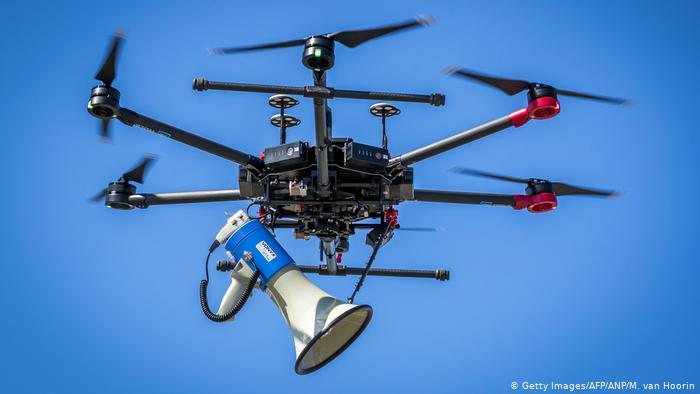
\includegraphics[width=\columnwidth]{drones.jpg}\\
	\caption{Drones used for announcements}\label{drones}
\end{figure}

Tunisia has deployed police robots on lockdown patrol \cite{tunisia}. These robots have proved to be really useful as they engage with all people coming outside to know the reason of their coming outside and do all the communication with the commands of police officials controlling it. But there are some issues with this robot like many people can easily escape from the robot, this can not keep a check on vehicles coming outside and we can not verify if one came outside for a really genuine reason or he/she is just lying to not get penalised.

\begin{figure}[!htb]
	\centering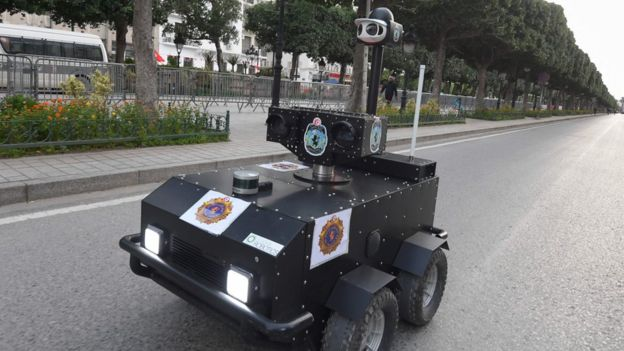
\includegraphics[width=\columnwidth]{tunisia.jpg}\\
	\caption{Robot used in Tunisia for patrolling}\label{robo}
\end{figure}

%-------------------------------------------------------------------------

\section{Blackboxes Used}
Following are the short descriptions of blackboxes used in our idea.
\subsection{YOLO Algorithm}
 YOLO algorithm is single convolutional network which simultaneously predicts multiple bounding boxes and class probabilities for those boxes \cite{yolo}. YOLO trains on full images and directly optimizes detection performance. 
 
 \subsection{FaceNet Algorithm}
 FaceNet provides a unified embedding for face recognition, verification and clustering tasks. It maps each face image into a euclidean space such that the distances in that space correspond to face similarity, i.e. an image of person A will be placed closer to all the other images of person A as compared to images of any other person present in the dataset  \cite{Schroff_2015}.
 
 \subsection{OCR}
 Optical character recognition or optical character reader (OCR) is the electronic or mechanical conversion of images of typed, handwritten or printed text into machine-encoded text, whether from a scanned document, a photo of a document, a scene-photo (for example the text on signs and billboards in a landscape photo) or from subtitle text superimposed on an image (for example from a television broadcast) \cite{ocr}.For a system of the automatic number plate recognition with OCR, it needs to have six algorithm processes to detect the plate data properly. The first algorithm would be the plate localization, which is the process of responsibly finding the plate on the image captured on the screen. The second would be the plate orientation and sizing. This is the process that will compensate for the skew and adjust the dimensions to get the desired image size. Furthermore, found in the automatic number plate recognition with OCR, is the normalization, character segmentation and geometrical analysis algorithms. The last algorithm and system would be the optical character recognition.
%-------------------------------------------------------------------------

\section{System Architecture}
\textbf{RemotePolice} is a software system application which will be authored to be used only by police officials. We will deploy robots at various locations of a city in such a way that all major portions of the city gets covered by these robots. In such a way we will create a robot network in the city. Also this idea will require us to have a database of images of all people of certain place along with their proper details which can be further used in face recognition task and a database storing vehicle owners for all vehicle number plates which will be used to get owner details from number plate of a vehicle.
\subsection{Robots}
Our robots will cover full city creating a network. Each robot will be attached with two different cameras for different purpose. 

\subsubsection{First Camera}
First camera will be used for detecting various objects around it through object detection \textbf{YOLO} algorithm, this will detect vehicles and pedestrians.

\begin{figure}[!htb]
	\centering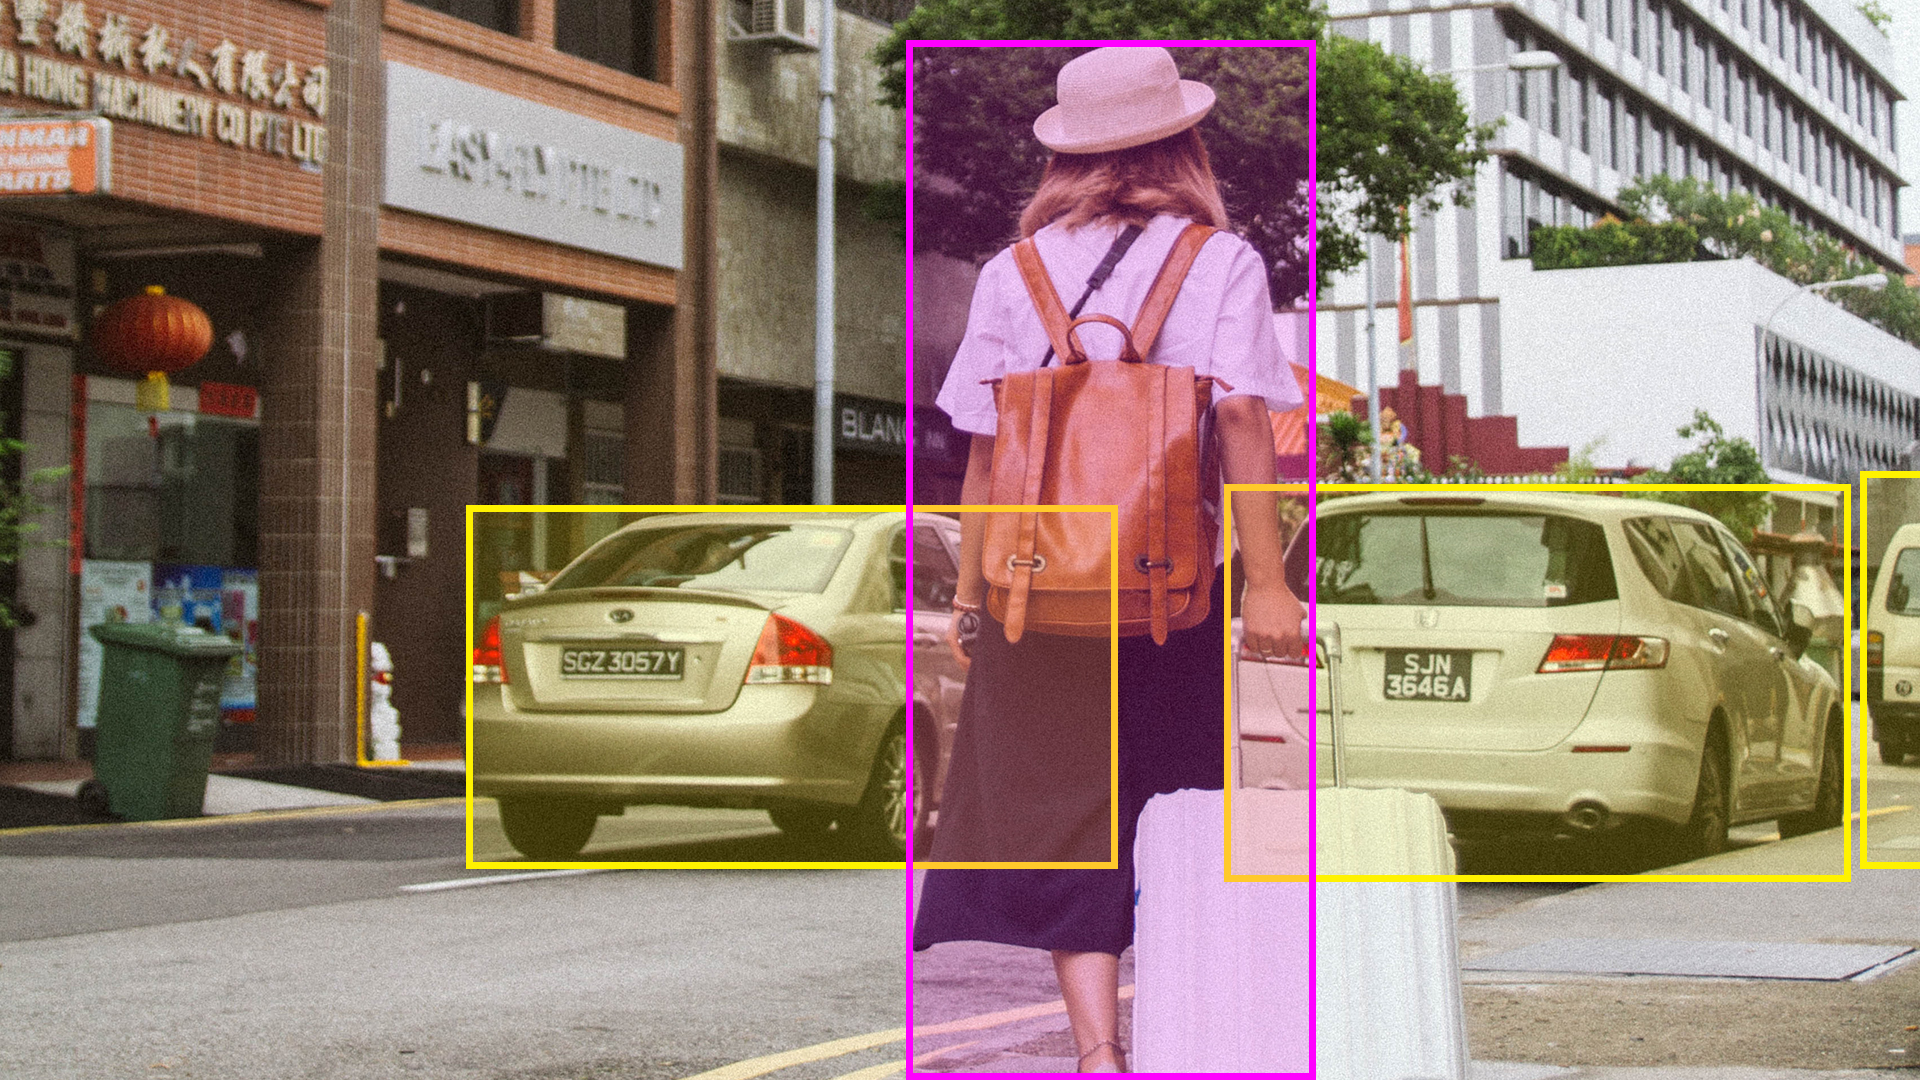
\includegraphics[width=\columnwidth]{object_detection}\\
	\caption{Detection of Pedestrian and vehicles using YOLO algorithm}\label{object_detection}
\end{figure}


\begin{figure*}
  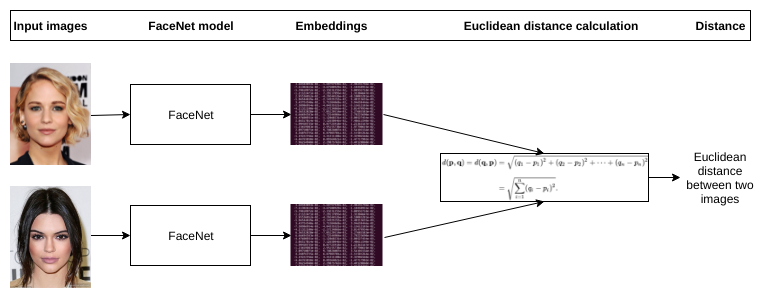
\includegraphics[width=\textwidth]{facenet.png}
  \caption{FaceNet Algorithm}
\end{figure*}

If detected object would be a pedestrian then robots cameras will focus to capture the face of pedestrian and after that using \textbf{FaceNet} algorithm our robot will try to recognize that face with help of our current database of all people. After the recognition task details of person recognized will be saved in a new database \textbf{Suspected}, which will store details of all people who came outside. The stored details in this database will include Name, Contact Number, Address, location and time where the person was seen.


If detected object would be a vehicle then robot cameras will focus to capture the number plate of the vehicle and after that using \textbf{OCR}(Optical Character Recognition) algorithm robot will read the number of the vehicle from number plate. Then from the database of vehicle's number plates we will get the details of the person owning the vehicle and similarly save all details of that person in the \textbf{Suspected} database.

\begin{figure}[!htb]
	\centering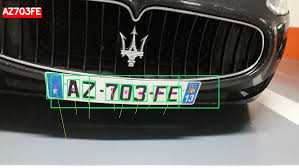
\includegraphics[width=\columnwidth]{ocr}\\
	\caption{OCR of number plate}\label{ocr}
\end{figure}

\subsubsection{Second Camera}
The role of second camera would be to interact with people. Our robot will go to all pedestrians detected outside and will start a conversation with them. From robot end it will speak whatever police will speak in the microphone of device in which police official is using our software to control this robot. In this way police will engage in a communication with the pedestrian remotely and will get all details they want like why pedestrian have came outside etc. If pedestrian claims that he has official pass to come outside then he/she will be asked to show the pass to camera attached to robot which will be verified by the police official. 

If police finds pedestrian's reason to be valid he/she will be allowed to go and his entry will be removed from the \textbf{Suspected} database. In this way robots will help police to communicate with pedestrians remotely and also note down the details in the database if someone's reason not seems valid or if someone escapes from robot's conversation.

\subsection{Verification of Person's Destination}
\label{sec:ver}
Now one major issue with the idea till now is that this system will penalise those people too who came outside for some essentials purpose eg. if a person needs to go to a doctor urgently our system will note his car's number too in the database and will penalise them. 

To take this into account as mentioned earlier we stored time and location also of each person/vehicle detected. So as the details of every vehicle will be stored in the database in increasing order of time of detection we can easily map the path of a vehicle as we know at what time it was noticed at what place. So when police will query that person on the call they will ask them reason to come out and if they claim that they went to some doctor urgently or for some other very important purpose, police can easily verify if they went to certain location or not as they have complete detail of that vehicle in order of time. With this timely data of location of a vehicle police officials can easily map full path followed by vehicle therefore getting where that vehicle travelled. So by this way if the reason of that person is valid he will be relieved from penalty or else police will impose certain penalty on the person depending on the situation.

With the help of extensive database police will also be able to know the frequency of each person coming outside so they can take actions accordingly.

\begin{figure}[!htb]
	\centering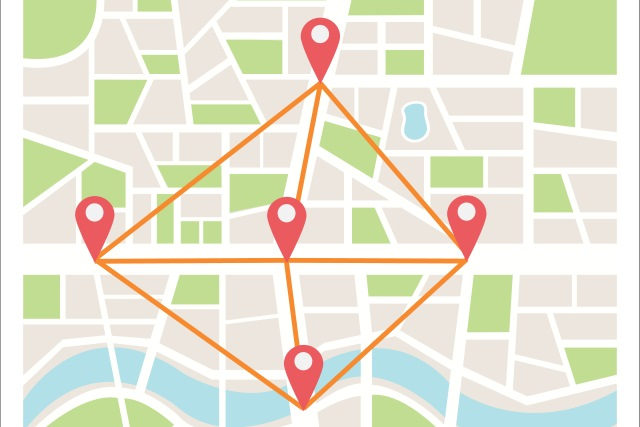
\includegraphics[width=\columnwidth]{path.jpeg}\\
	\caption{This diagram shows positions of a particular vehicle noticed at various times. Using this we can frame exact path travelled by that vehicle}\label{path}
\end{figure}


\subsection{MVC architecture}
The MVC architecture pattern  divides an  application interaction  into three  components\cite{mvc}. The model contains the  functions and  core data. View  shows information to the user.  The controller handles  user input. View and controller are both composed of the user interface. MVC follows the most common approach to Layering. Layering is just a logic that divides our code into functions  into different classes. This approach is easily recognized and the most widely accepted. The main advantage of this approach is the reusability of the code

\begin{figure*}
  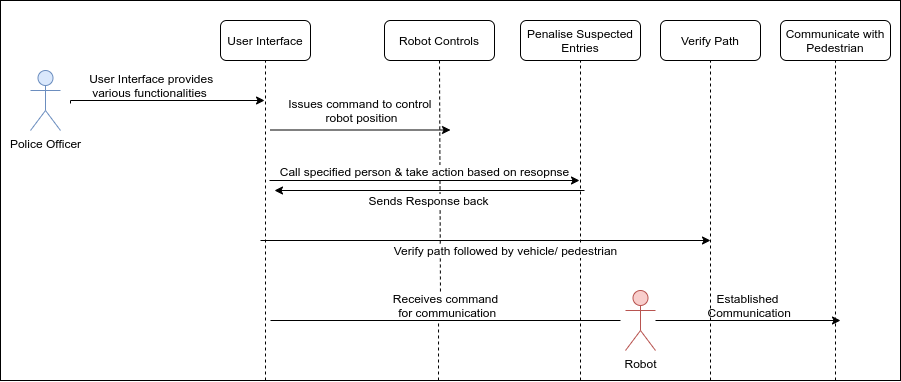
\includegraphics[width=\textwidth]{sequence.png}
  \caption{UML sequence diagram for software application}
\end{figure*}

\subsubsection{Model}
For our software application we will use three databases(models) for different purpose.
\paragraph{Face Image Database}
This database will store image of faces of all people of a region along with their proper details. We will use this database for purpose of facial recognition task to get the details of detected pedestrian.
\paragraph{Number Plate Database}
This database will store vehicle number of all vehicles of a certain region along with proper details of vehicle's owner. We will use this database when we need to extract details of vehicle owner from vehicle number at the time when robot will detect some vehicle.

\paragraph{Suspected}
This will be the database in which we will store details of all pedestrians and vehicle owners detected outside by our robots. This will be used by application user i.e police officials. From this database police will see who all came outside and then they will contact them for penalising them. Also this database will store proper details of vehicles along with location and time of their detection, using which police can easily confirm where a particular vehicle travelled as explained in above \emph{Verification of Person's Destination} section \hyperref[sec:ver]{[1]}. Upon verification of a person police would also be able to remove entry from this database.


\subsubsection{Controller}
Controller is a component that serves to call the function in the model and send the results through View, Controller also take input from the user which will then be processed by Model. Thus, the controller is responsible for mapping the final user action against the application response. When a request arrives on the server, the MVC framework sends it to a method in the controller. Following are functions in our controller part:
\paragraph{Handle Position} Using this function police can control position and cameras of robot remotely so that robot can detect cases more accurately.
\paragraph{Call} Through this function police can communicate remotely with pedestrian. Police will need to speak in the microphone of device having software application to send his message. This function will be called when robot detects some pedestrian and gets command from police to go near the pedestrian and start the communication.
\paragraph{Scanner} This function will show police the view of scanner camera of robot. This scanner camera will be used if pedestrian detected wants to show some document/pass to police. Through these documents police can verify that person.
\paragraph{See suspected one's} Through this function police officer will be able to get details all the pedestrians and vehicles detected outside present in \emph{Suspected} database. Using these details police will contact all suspected people and ask them about reason for coming outside and  will give penalty accordingly.

\paragraph{Delete Entry} Through this function police will be able to delete some entry from \emph{Suspected} database.

\begin{figure*}
  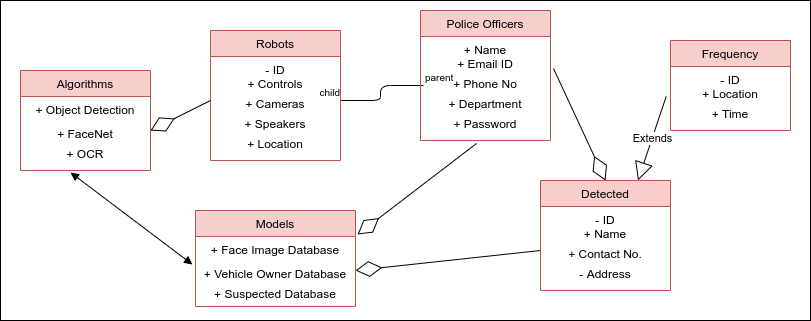
\includegraphics[width=\textwidth]{uml.png}
  \caption{UML diagram for software application}
\end{figure*}

\paragraph{Verify Destination} This function will be used when police wish to check where a vehicle travelled. This can be used by police while he is asking a suspected person about why they came out and they in response tell that they went to some place for some important purpose. In order to verify if the person is not lying police can use this function which will return the location of all detected cases of that particular vehicle or person in order of increasing time. Using this list police can easily frame full travel path of that vehicle and can verify if it has travelled to a certain place or not.

\paragraph{Statistics} Using this function police can see overall data in graphical form of how many people are coming outside in a certain region.
\paragraph{Specific Details} Using this function police can see specific details of a single person about his frequency of coming outside.
\subsubsection{View}
As this software application has not been implemented so we can not tell anything about view part.

\begin{figure*}
  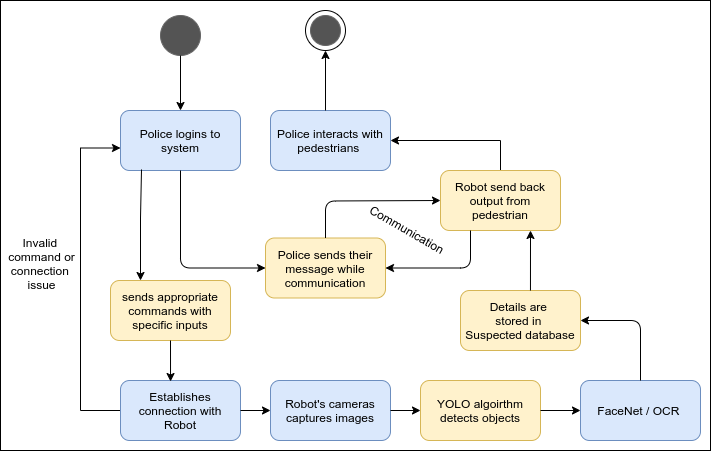
\includegraphics[width=\textwidth]{uml_state.png}
  \caption{UML state diagram for software application}
\end{figure*}

\subsection{Actors}
We will allow only police officials to register and control robots for their region, therefore different officials will be allocated for control of each robot, which will result in seamless flow of the entire system.

\subsection{Use Cases} 
Our application will offer following use cases to police officers:
\begin{itemize}
    \item Police can control the position of robot and its cameras.
    \item  Police will be able to have a communication with the pedestrians remotely, they will speak in the microphone and will have a communication through the robot.
    \item  Police will be able to view the details of all people who came outside in a proper format along with their frequency of coming out.
    \item  They can contact the person and based upon his response and our verification system can mark his reason as genuine or not and based upon that can penalise them.
\end{itemize}

\subsection{Advantages of MVC Design Pattern}
MVC is important to understand because it is the basic structure which most web applications are built on. 
\begin{itemize}
\item Development of the application becomes fast.
\item Easy for multiple developers to collaborate and work together.
\item Easier to Update the application.
\item Easier to Debug as we have multiple levels properly written in the application.
\end{itemize}

\begin{figure*}
  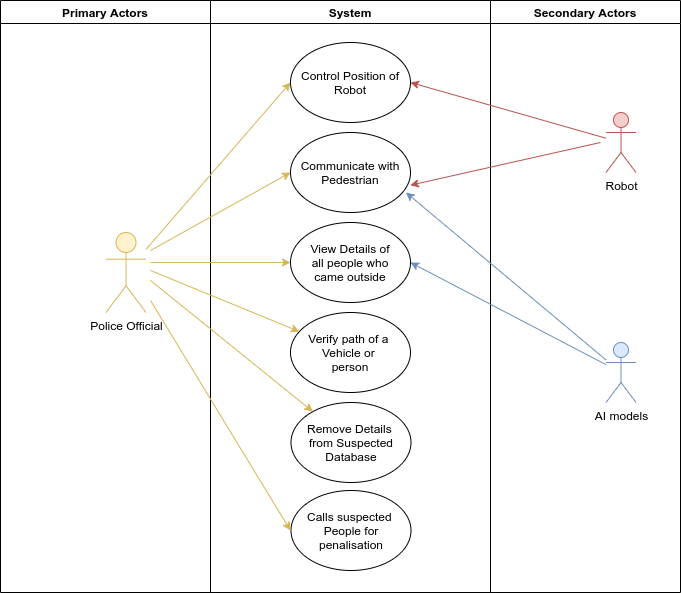
\includegraphics[width=\textwidth]{usecase.png}
  \caption{Use Case diagram for software application}
\end{figure*}


\section{Conclusion and Future Work}
Along with the implementation and testing of the entire system we can get some challenges and exceptions for which we may need to find some alternative ways or some more efficient approach. Our future work will include implementing this whole system and finding solution to all such challenges and exceptions we face. It would require some time and effort for the implementation of the entire system, but with a great team it can be done in a very efficient manner. It would also require a large support from the government to implement such a system in the society. But on the whole if we can establish all the supports and fulfill all the requirements, \textbf{RemotePolice} would be proved as the best solution for this problem in the society.

{\small
\bibliographystyle{ieee}
\bibliography{egbib}
}

\end{document}
